\documentclass[/home/jesse/Analysis/FemtoAnalysis/AnalysisNotes/AnalysisNoteJBuxton.tex]{subfiles}
\begin{document}

\subsection{Results: \texorpdfstring{$\Xi$K$^{\pm}$}{TEXT}}
\label{ResultsXiK}

Even without any fits to the data, the fact that the $\Xi^{-}$K$^{+}$ data dips below unity (Fig. \ref{fig:XiKchwConjResults}) is exciting, as this cannot occur purely from a Coulomb interaction.  We hope that this dip signifies that we are able to peer through the overwhelming contribution from the Coulomb interaction to see the effects arising from the strong interaction.

\begin{figure}[h]
  \centering
  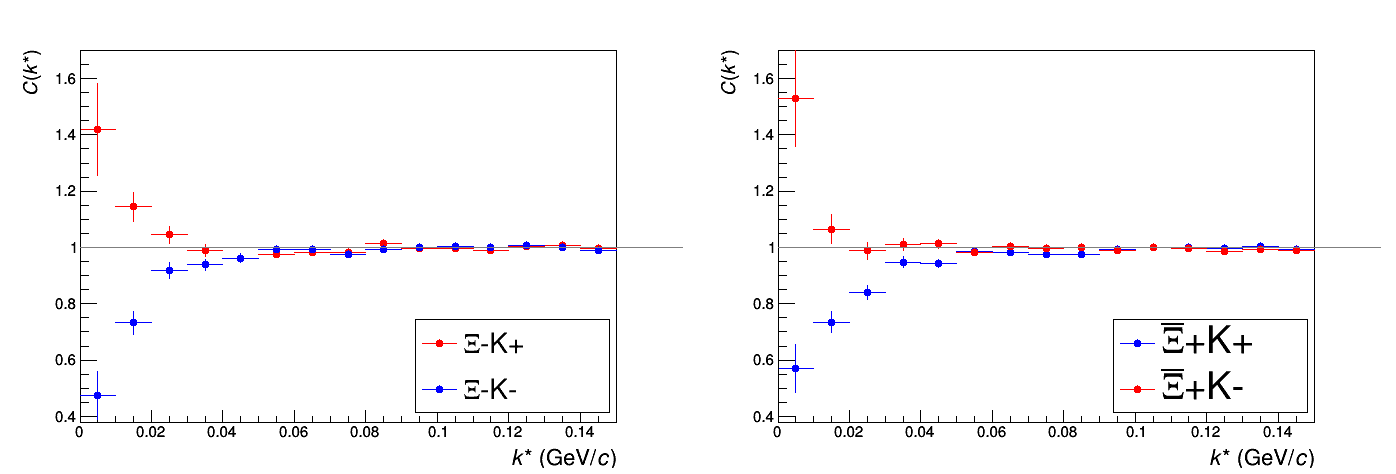
\includegraphics[width=\textwidth]{7_ResultsAndDiscussion/Figures/cXicKchKStarCfs.png}
  \caption[$\Xi$K$^{\pm}$ Results]{$\Xi$K$^{\pm}$ Results for 0-10\% Centrality.  (Left) $\Xi^{-}$K$^{+}$ and  $\Xi^{-}$K$^{-}$  (Right) $\bar{\Xi}^{+}$K$^{+}$ and  $\bar{\Xi}^{+}$K$^{-}$}
  \label{fig:XiKchwConjResults}
\end{figure}

%%%%%%%%%%%%%%%%%%%%%%%%%%%%%%%%%%%%%%%%%%%%%%%%%%%%%%%%%%%%%%%%%%%%%%%%%%%%%%%%%%%%%%%%
\begin{comment}
\begin{figure}[h!]
  \centering
  %%----start of first subfigure---  
  \subfloat[$\Xi$K$^{+}$ First Fit, 0-10\% Centrality]{
    \label{fig:XiKchFits:a}
    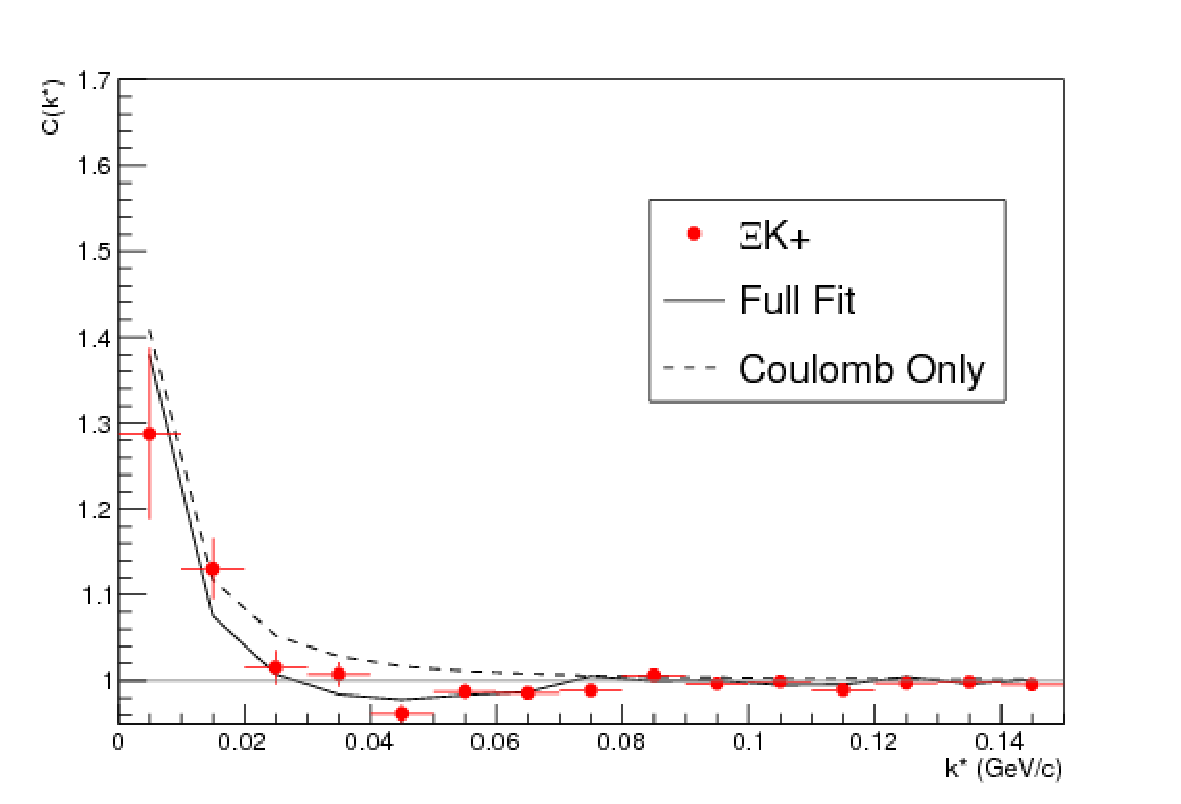
\includegraphics[width=0.49\textwidth]{7_ResultsAndDiscussion/Figures/XiKchP.pdf}}
  %%----start of second subfigure---
  \subfloat[$\bar{\Xi}$K$^{+}$ First Fit, 0-10\% Centrality]{
    \label{fig:XiKchFits:b}
    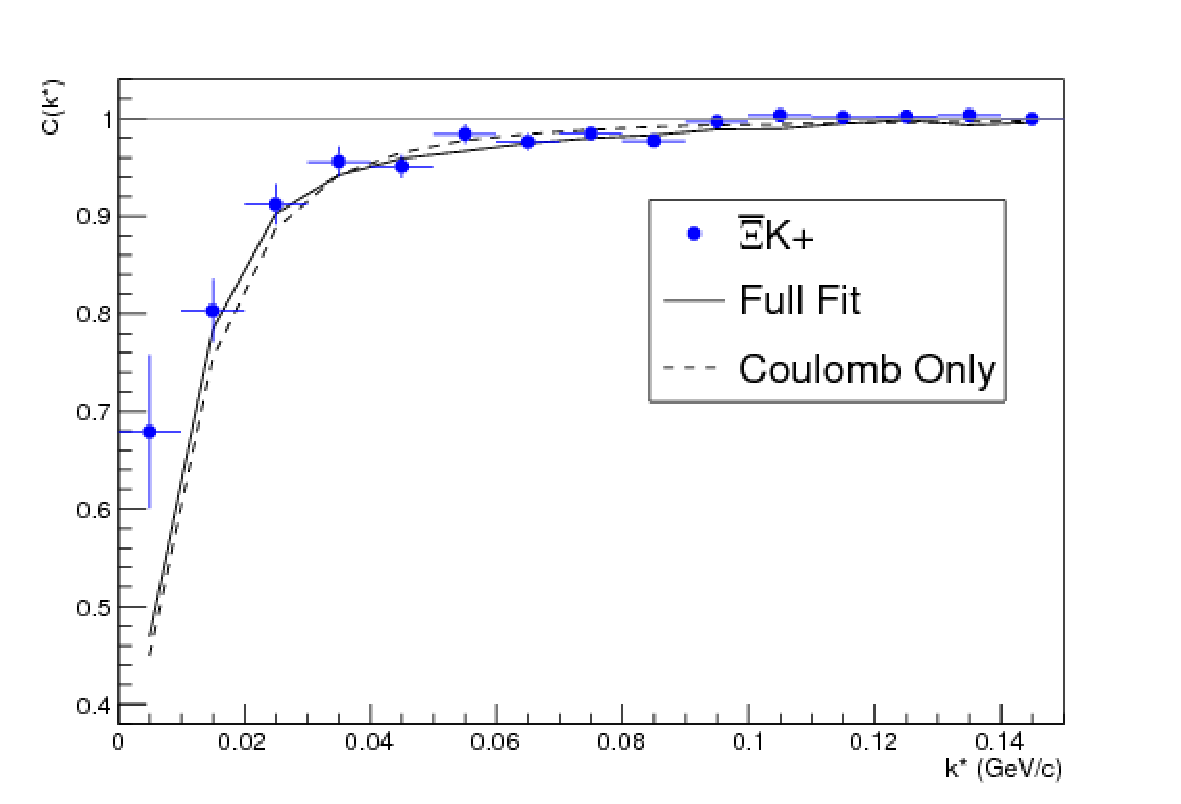
\includegraphics[width=0.49\textwidth]{7_ResultsAndDiscussion/Figures/AXiKchP.pdf}}
  %%----overall caption----
  \caption[$\Xi$K$^{\pm}$ First Fits]{$\Xi$K$^{\pm}$ First Fits}
  \label{fig:XiKchFits}
\end{figure}
\end{comment}
%%%%%%%%%%%%%%%%%%%%%%%%%%%%%%%%%%%%%%%%%%%%%%%%%%%%%%%%%%%%%%%%%%%%%%%%%%%%%%%%%%%%%%%%

Figure \ref{fig:XiKchCoulombOnlyBand} demonstrates graphically, that the $\Xi^{-}$K$^{+}$ results cannot be described by solely the Coulomb interaction.  In this figure, we present the data along with a Coulomb-only band.  The Coulomb-only band is spanned by two Coulomb-only curves, whose parameters are given in the figure. The Coulomb-only curves were generated using a technique identical to the generation of the fit function, described in Sec. \ref{ModelCascadeKaon}, except, of course, with the nuclear scattering parameters all set to zero.  The Coulomb-only curves change monotonically with varying $\lambda$ or varyin radius parametres, therefore, any curves built with parameter sets intermediate to those use in the Coulomb-only band will be contained in the band.

\begin{figure}[h]
  \centering
  %%----start of first subfigure---  
  \subfloat[(Left) $\Xi$K$^{+}$ and (Right) $\bar{\Xi}$K$^{-}$]{
    \label{fig:XiKchCoulombOnlyBand:a}
    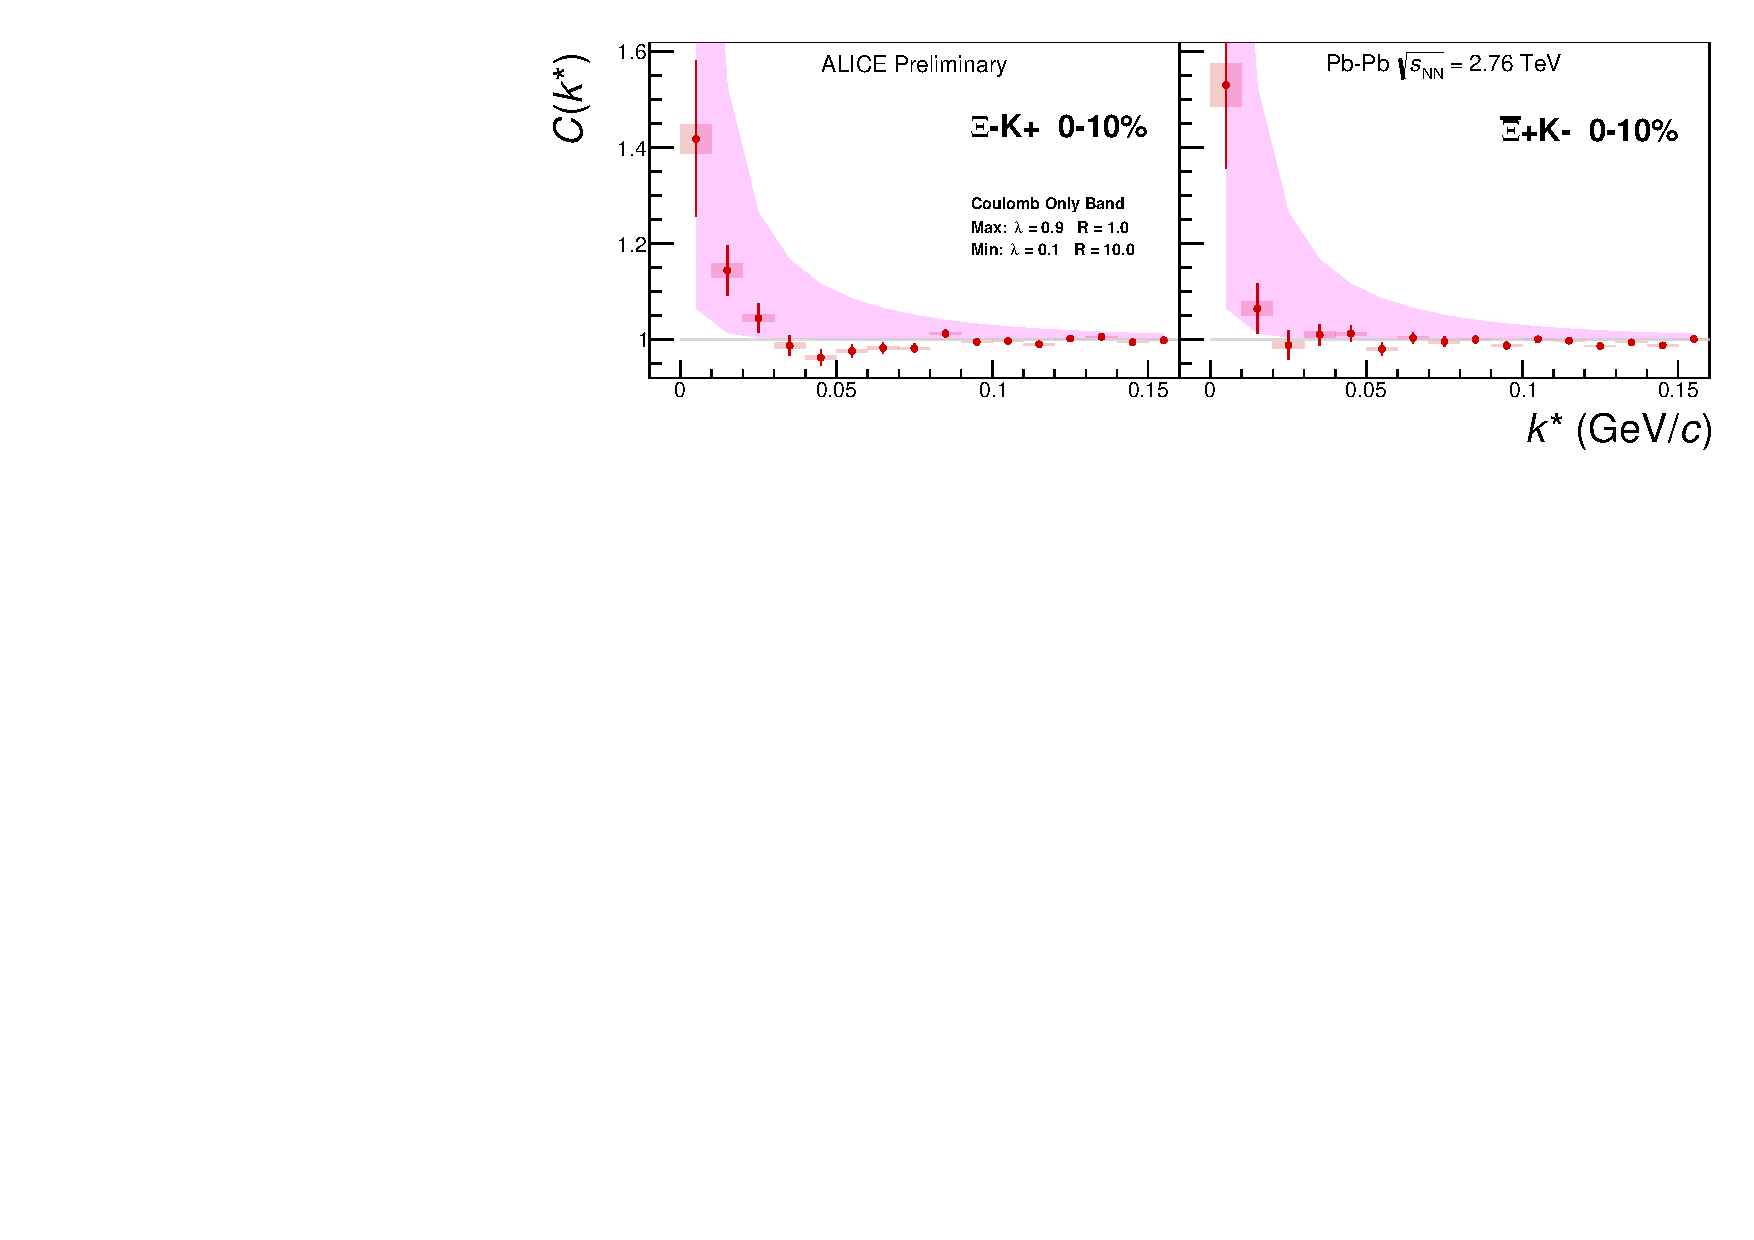
\includegraphics[width=0.99\textwidth]{7_ResultsAndDiscussion/Figures/WPCFCoulombOnlyCurves_XiKchP_0010_Stretch.pdf}}\\
  %%----start of second subfigure---
  \subfloat[(Left) $\Xi$K$^{-}$ and (Right) $\bar{\Xi}$K$^{+}$]{
    \label{fig:XiKchCoulombOnlyBand:b}
    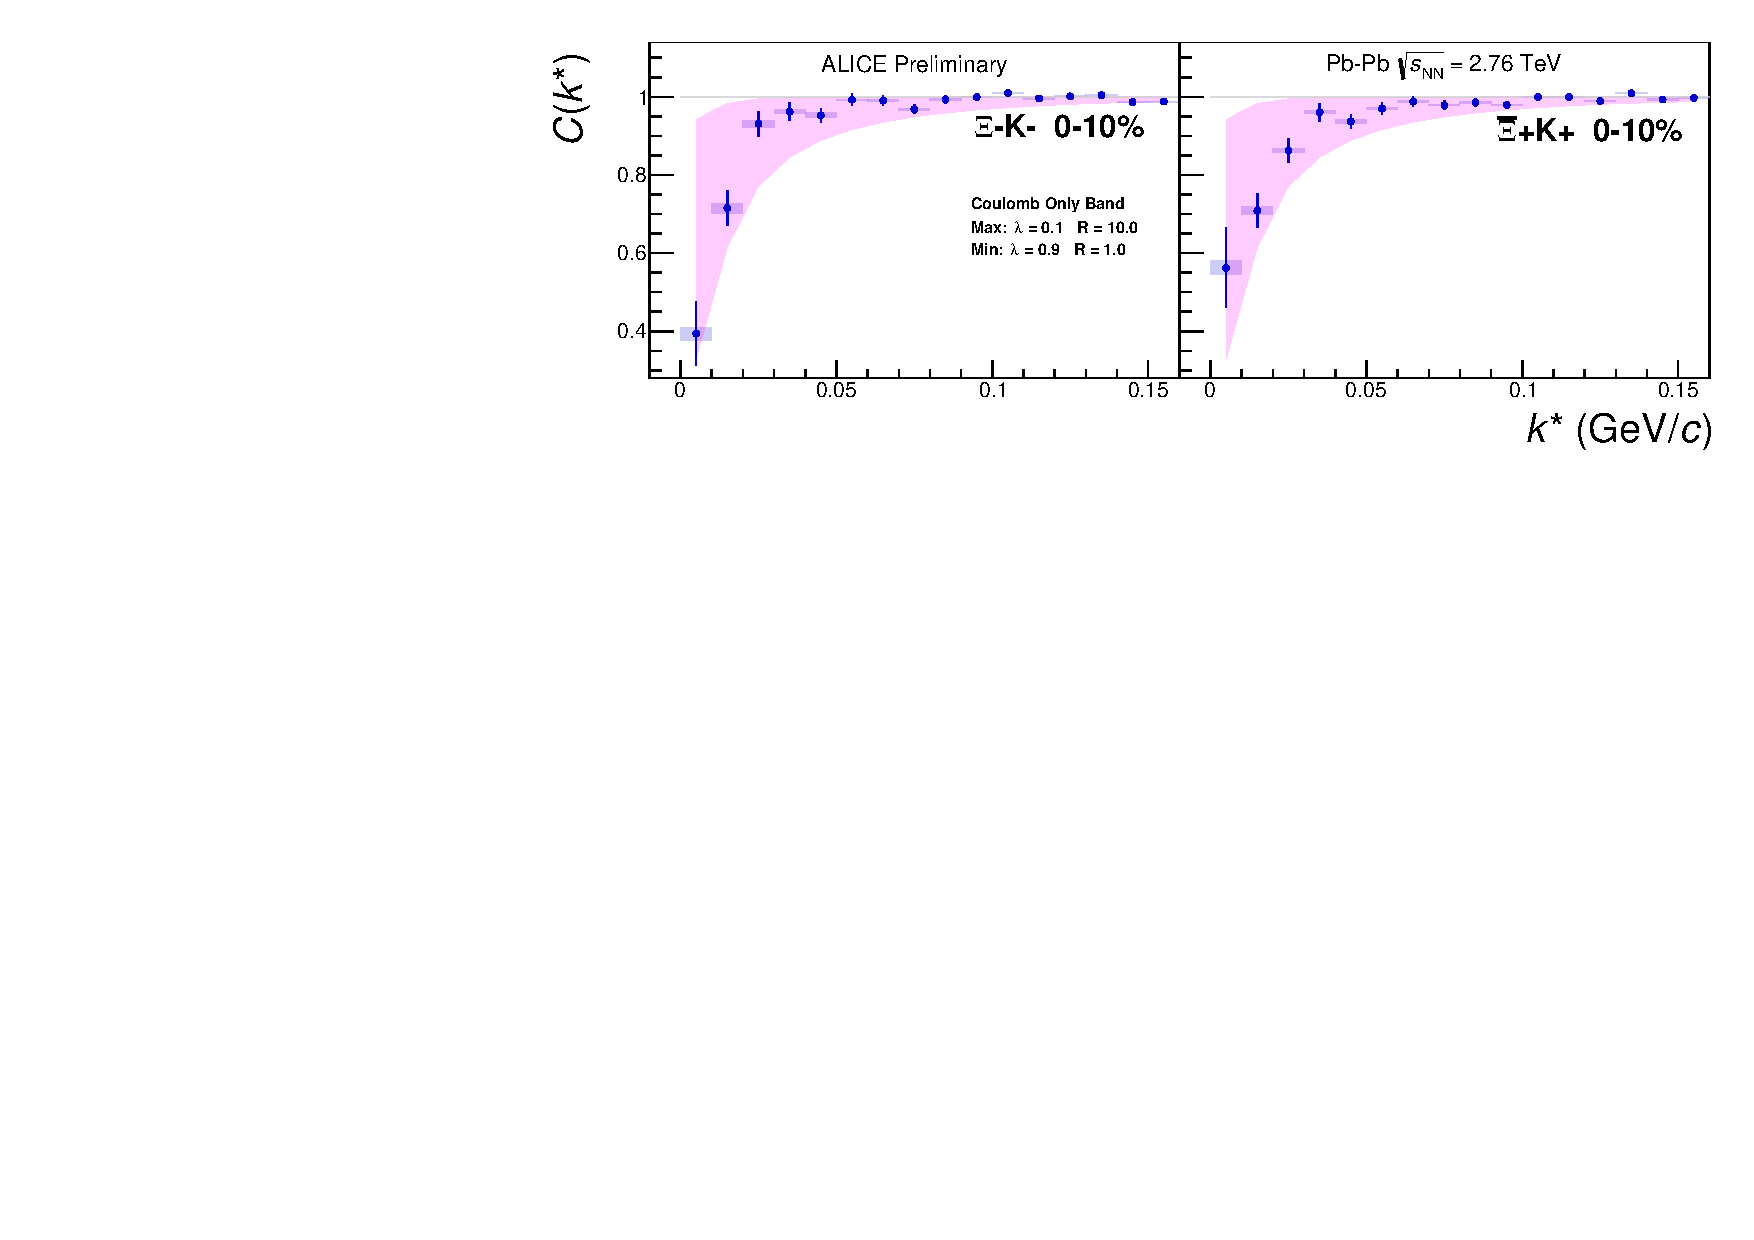
\includegraphics[width=0.99\textwidth]{7_ResultsAndDiscussion/Figures/WPCFCoulombOnlyCurves_XiKchM_0010_Stretch.pdf}}
  %%----overall caption----
  \caption[$\Xi$K$^{\pm}$ Data with Coulomb-Only Bands, 0-10\% Centrality]{$\Xi$K$^{\pm}$ data with Coulomb-only bands for the 0-10\% centrality bin.  The Coulomb-only bands span two sets of Coulomb-only curves: (1) $\lambda$ = 0.9, R = 1.0 fm and (2) $\lambda$ = 0.1, R = 10.0 fm.  The Coulomb-only curves are simulated correlation functions for the respective pair system assuming only a Coulomb interaction, i.e. ignoring the strong interaction.  The Coulomb-only curves change monotonically with varying $\lambda$ and varying R, therefore, any intermediate parameter set will fall within this Coulomb-only band.}
  \label{fig:XiKchCoulombOnlyBand}
\end{figure}

Including the strong interaction into the simulation can change, sometimes dramatically, the resulting correlation function, as shown in Figure \ref{fig:XiKchStrongInfluence}.  In the figure, the solid line represents a Coulomb-only curve, i.e. a simulated correlation function with the strong interaction turned off.  The dashed lines represent a full simulation, including both the strong and Coulomb interactions.  The two dashed lines differ only in the real part of the assumed scattering length: positive in Set 1, and negative in Set 2.  In the top figure, for the $\Xi^{-}$K$^{+}$ simulation, we see that parameter set 2, with a negative real part of the scattering length, causes the simulated curve to dip below unity, as is seen in the data.  If there is a parallel to be drawn between this analysis and the $\Lambda$K analysis, we expect to see similar effects in the $\Lambda$K+ system and the $\Xi^{-}$K$^{+}$ systems.  In these systems, we could have an s$\bar{\mathrm{s}}$ annihilation picture.  Or, another possible way of thinking about these systems is in terms of net strangeness.  The $\Lambda$K$^{+}$ system has S=0, while the $\Lambda$K$^{-}$ has S=-2.  The $\Xi^{-}$K$^{+}$ has S=-1, while the $\Xi^{-}$K$^{-}$ has S=-3.

\begin{figure}[h]
  \centering
  %%----start of first subfigure---  
  \subfloat[$\Xi$K$^{+}$ and $\bar{\Xi}$K$^{-}$ simulation]{
    \label{fig:XiKchStrongInfluence:a}
    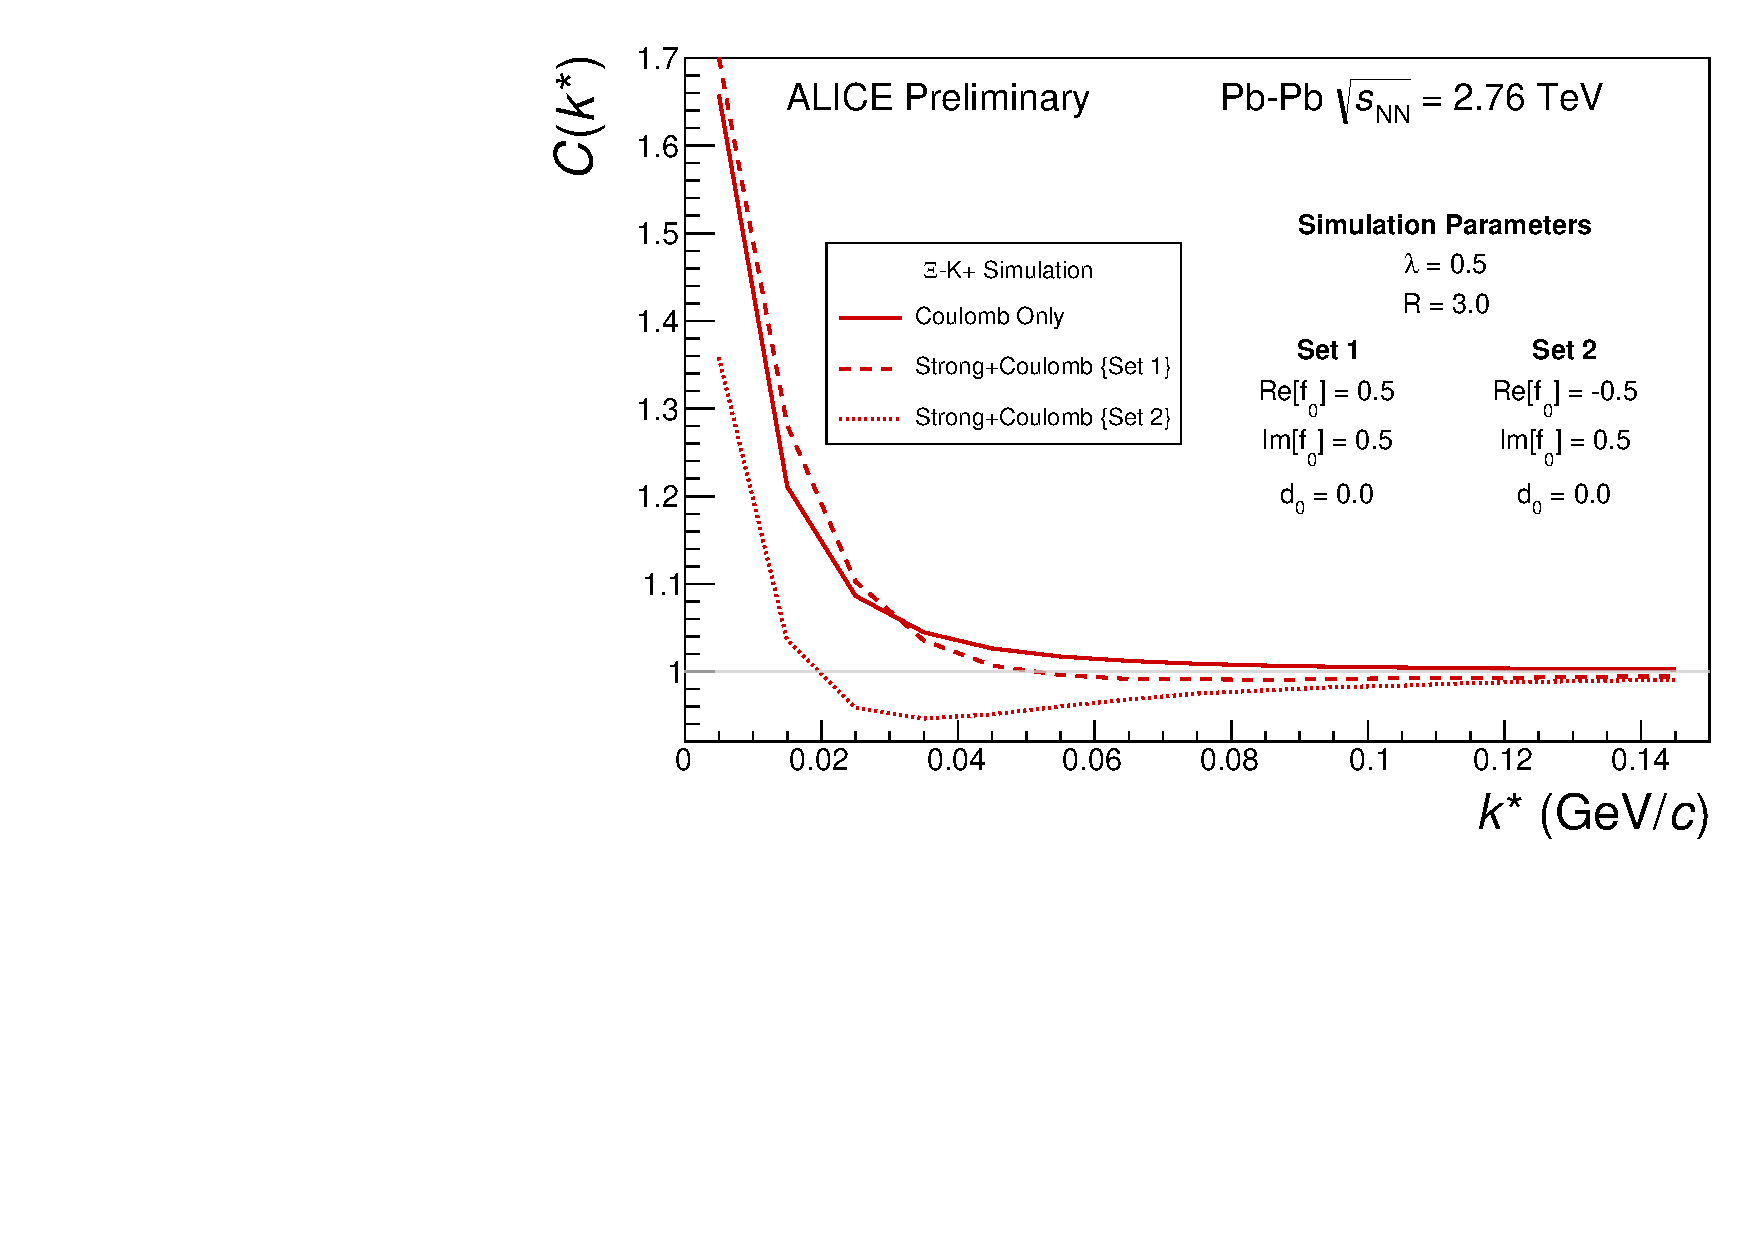
\includegraphics[width=0.99\textwidth]{7_ResultsAndDiscussion/Figures/WPCFStrongInfluence_XiKchP_0010_v2.pdf}}\\
  %%----start of second subfigure---
  \subfloat[$\Xi$K$^{-}$ and $\bar{\Xi}$K$^{+}$ simulation]{
    \label{fig:XiKchStrongInfluence:b}
    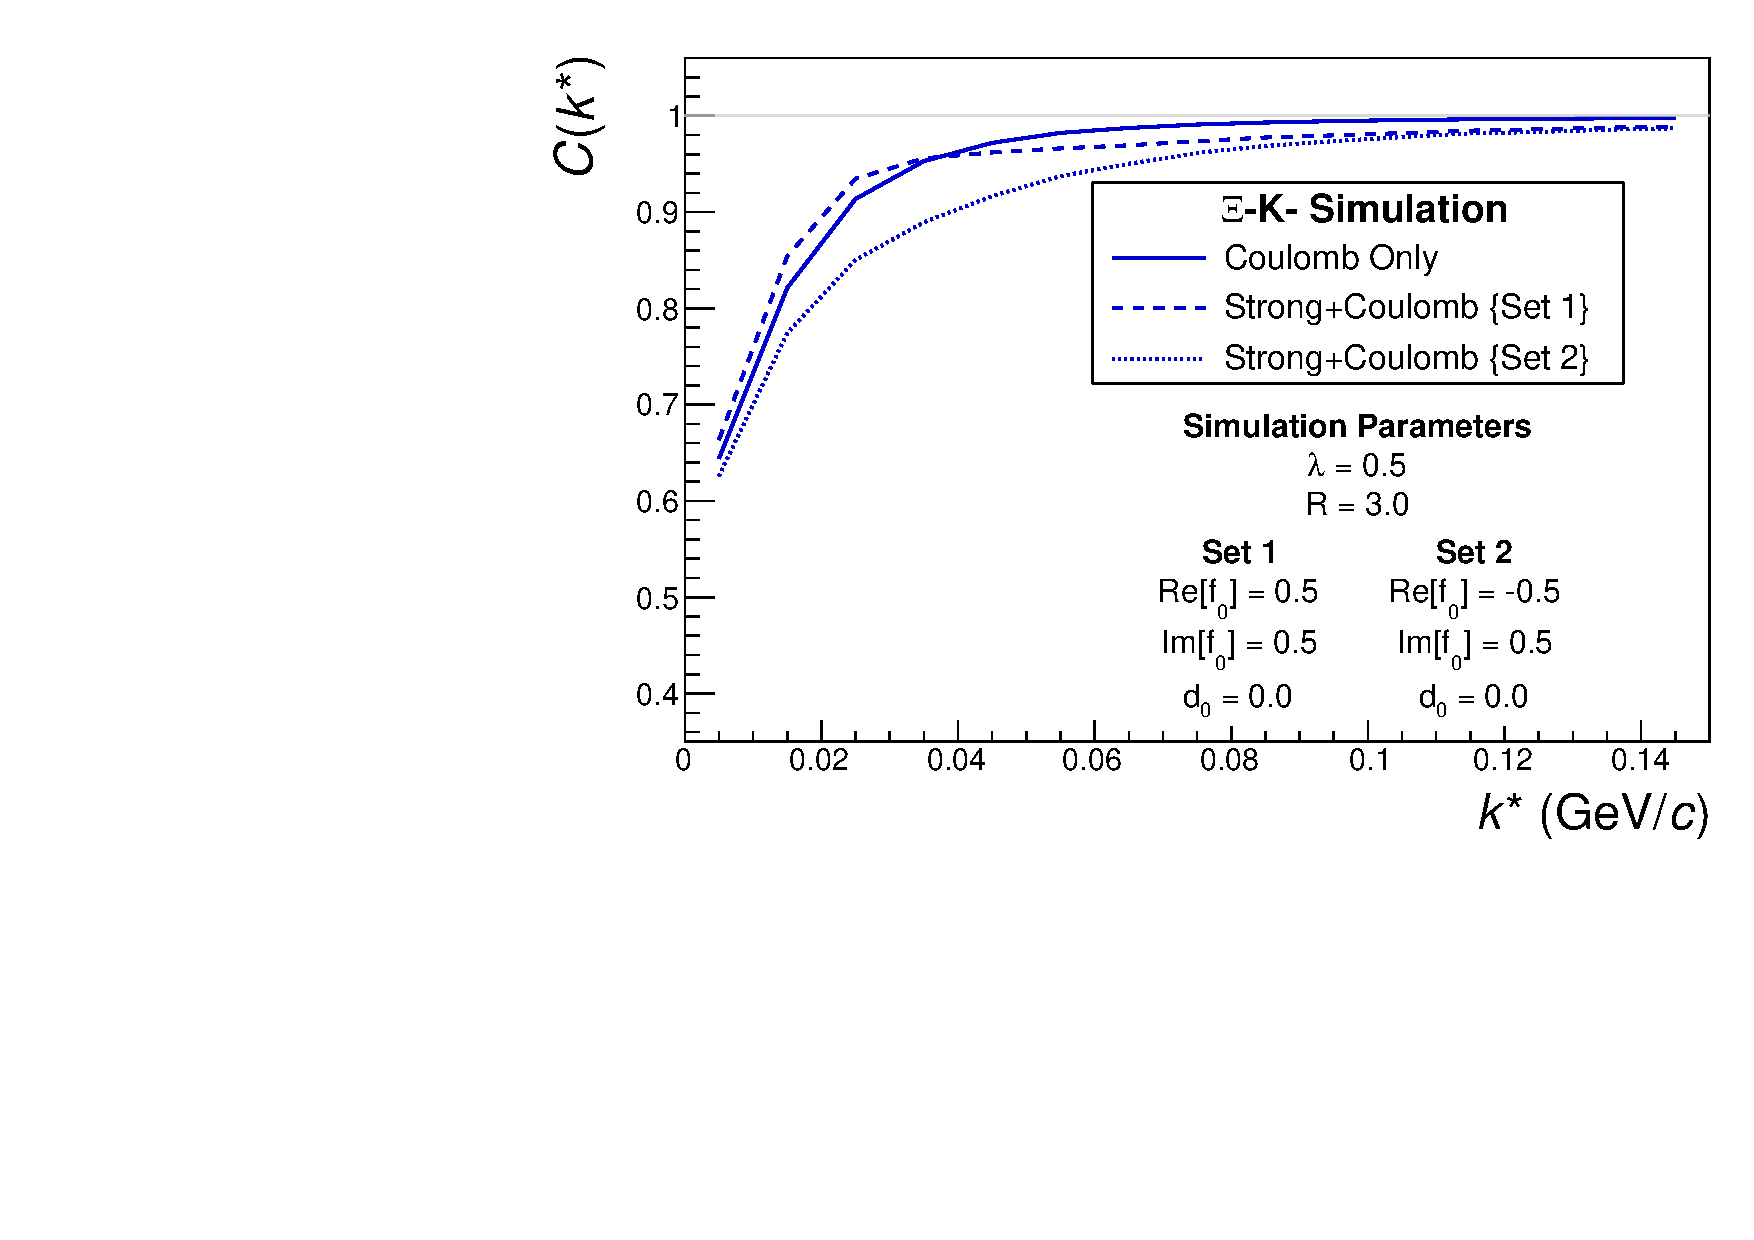
\includegraphics[width=0.99\textwidth]{7_ResultsAndDiscussion/Figures/WPCFStrongInfluence_XiKchM_0010_v2.pdf}}
  %%----overall caption----
  \caption[Effect of Strong Force Inclusion on Coulomb-Only Curve for $\Xi$K$^{\pm}$ systems]{Effect on the Coulomb-only curve of including the strong interaction for $\Xi$K$^{\pm}$ systems.  The solid line represents a Coulomb-only curve, i.e. a simulated correlation function with the strong interaction turned off.  The dashed lines represent a full simulation, including both the strong and Coulomb interactions.  The two dashed lines differ only in the real part of the assumed scattering length: positive in Set 1, and negative in Set 2.}
  \label{fig:XiKchStrongInfluence}
\end{figure}

The author was asked to perform a global Coulomb-only fit to the data, to ensure that the system truly could not be described simply by the Coulomb interaction.  In order words, in the fit, the strong force was turned off, and the $\Xi^{-}$K$^{+}$, $\bar{\Xi}^{+}$K$^{-}$, $\Xi^{-}$K$^{-}$, $\bar{\Xi}^{+}$K$^{+}$ systems all share one sinlge radius parameter, while the pair and conjugate pair systems share a $\lambda$ parameter.  The results of this fit are shown in Figures \ref{fig:XiKchGlobalCoulombOnlySet1} and \ref{fig:XiKchGlobalCoulombOnlySet2}.  In Fig. \ref{fig:XiKchGlobalCoulombOnlySet1}, there was a lower limit of 0.1 fm placed on the radius parameter, and the radius parameter was initialized to 3 fm (as seems reasonable, when considering the transverse mass of the system and looking at Fig. \ref{fig:mTScalingOfRadii}).  As is shown in the results, the radius parameter reached this unrealistic lower bound of 0.1 fm.  In Fig. \ref{fig:XiKchGlobalCoulombOnlySet2}, the parameters were all unbounded, and the radius parameter was initialized to 10 fm.  In this case, the radius parameters reamins high, and ends at an unrealistic value of 10.84 fm.  In both cases, the $\lambda$ parameters are too low.  From these figures, we conclude that a global Coulomb-only fit is not suitable for the data.

\begin{figure}[h]
  \centering
  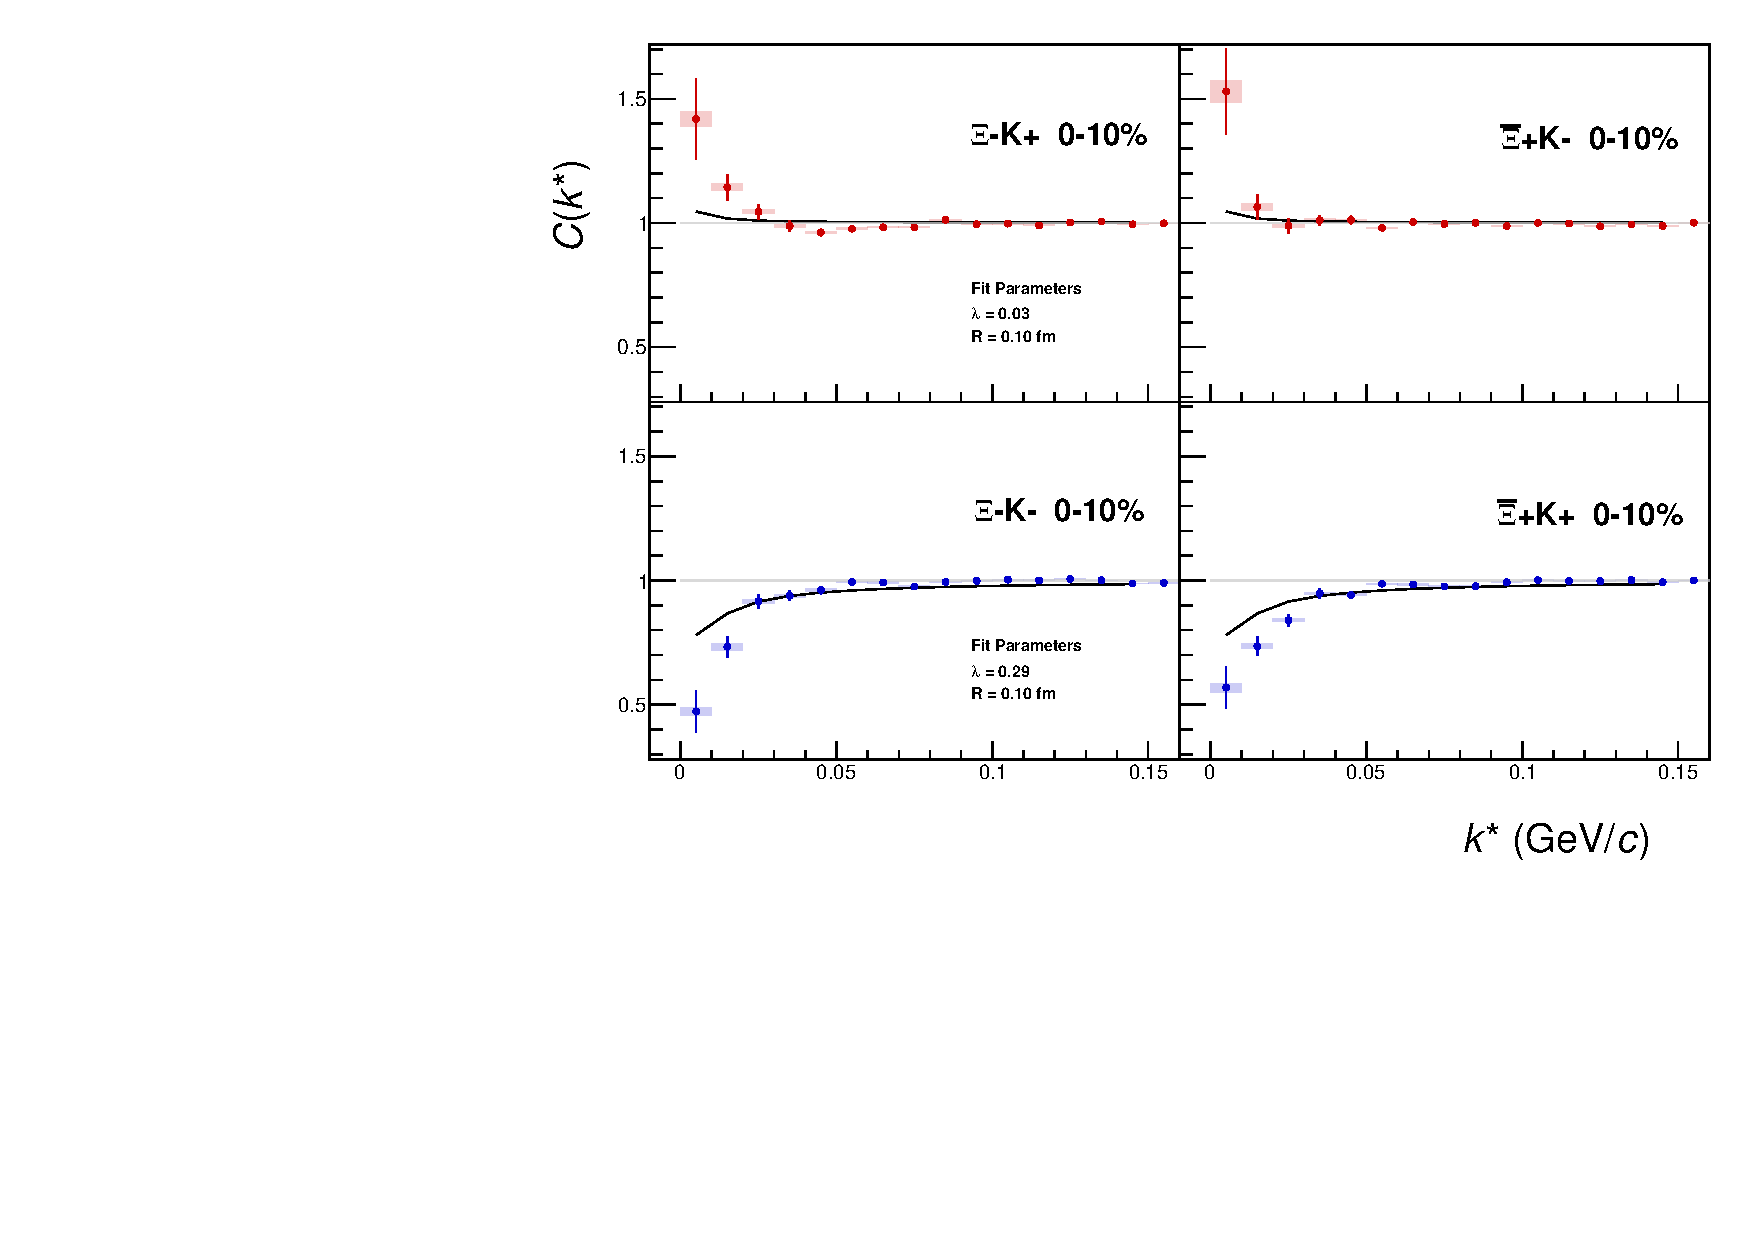
\includegraphics[width=\textwidth]{7_ResultsAndDiscussion/Figures/GlobalCoulombOnlyFit_Set1.pdf}
  \caption[$\Xi$K$^{\pm}$ Global Coulomb-Only Fit (Set 1)]{$\Xi$K$^{\pm}$ Global Coulomb-only fit (Set 1) for 0-10\% centrality.  In this fit, there was a lower limit of 0.1 fm placed on the radius parameter, and the radius parameter was initialized to 3 fm (as seems reasonable, when considering the transverse mass of the system and looking at Fig. \ref{fig:mTScalingOfRadii}).  As is shown in the results, the radius parameter reached this unrealistic lower bound of 0.1 fm.  Also, the extracted $\lambda$ parameters are too low.}
  \label{fig:XiKchGlobalCoulombOnlySet1}
\end{figure}

\begin{figure}[h]
  \centering
  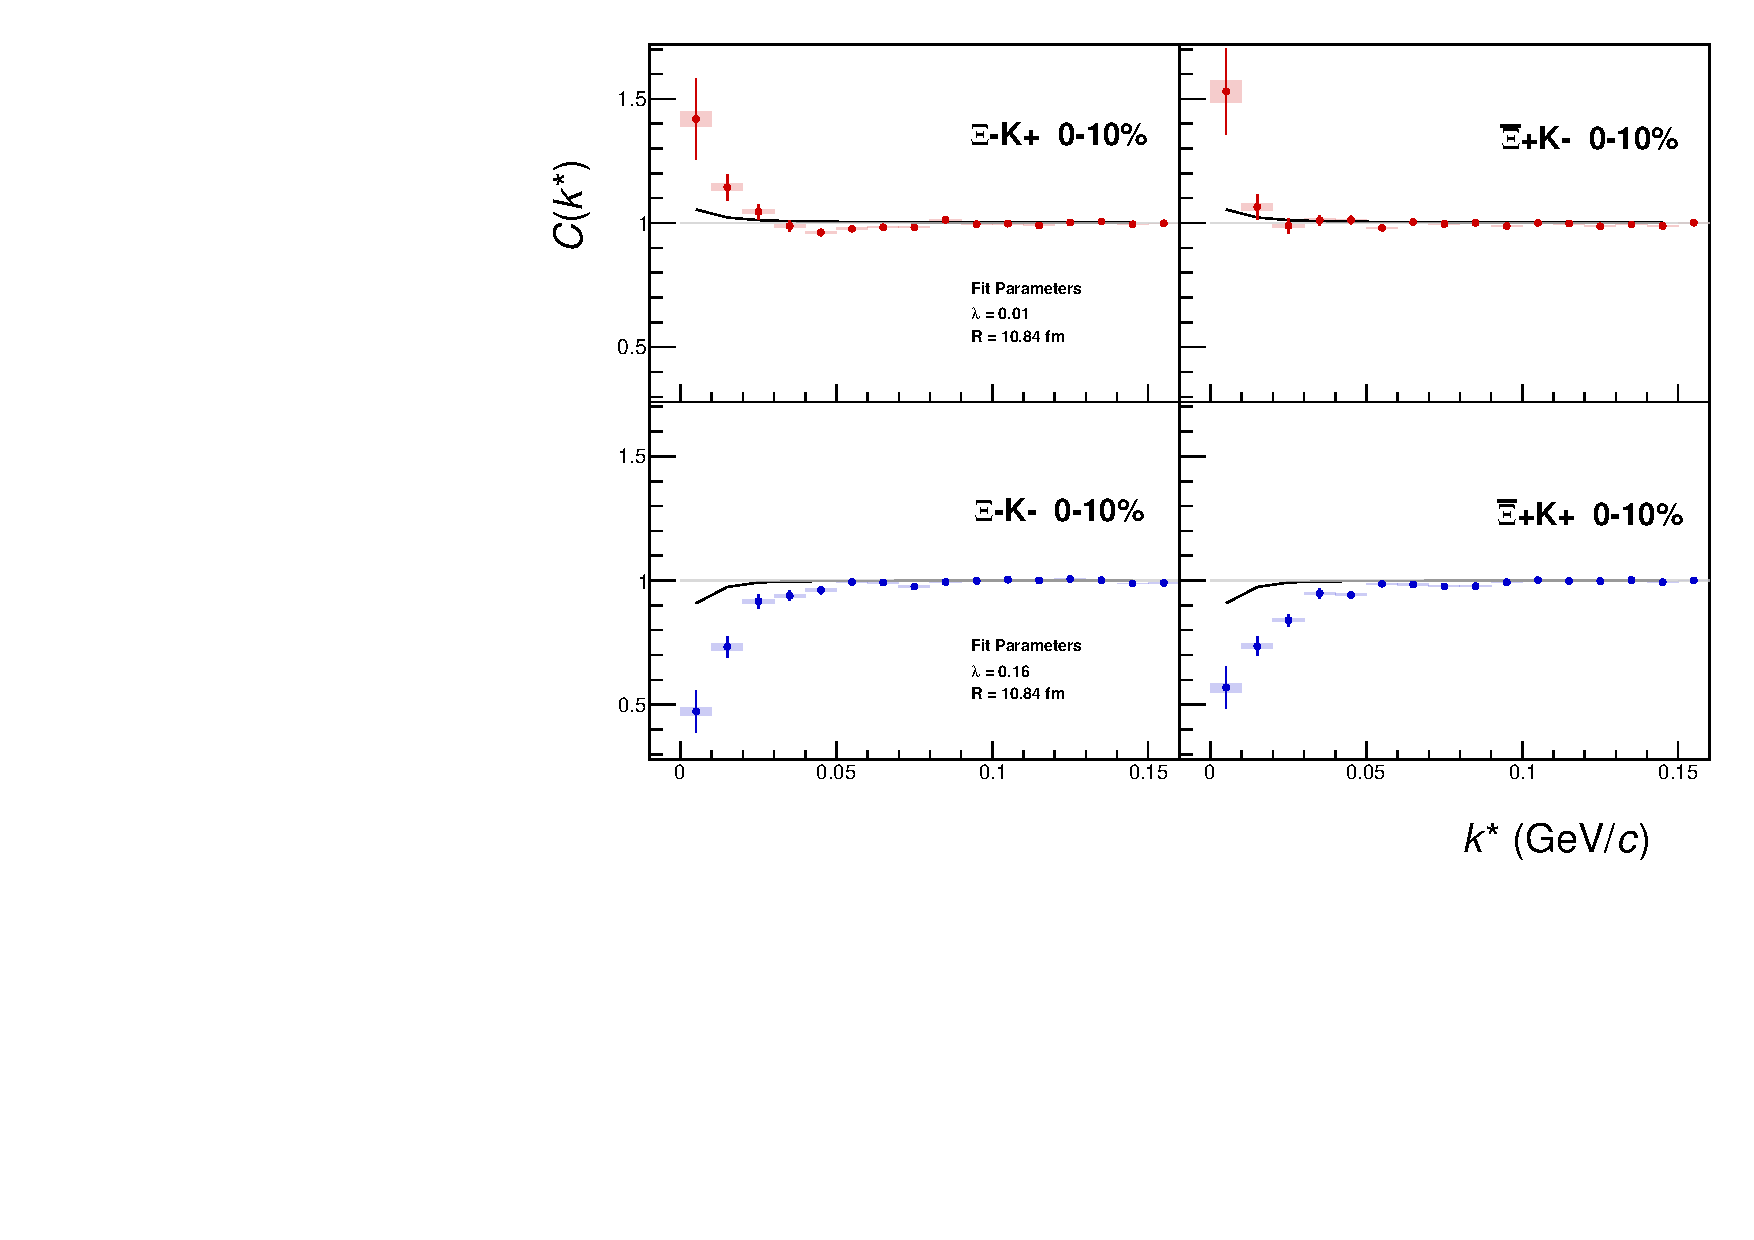
\includegraphics[width=\textwidth]{7_ResultsAndDiscussion/Figures/GlobalCoulombOnlyFit_Set2.pdf}
  \caption[$\Xi$K$^{\pm}$ Global Coulomb-Only Fit (Set 2)]{$\Xi$K$^{\pm}$ Global Coulomb-only fit (Set 2) for 0-10\% centrality.  In this fit, the parameters were all unbounded, and the radius parameter was initialized to 10 fm.  In this case, the radius parameters reamins high, and ends at an unrealistic value of 10.84 fm.  Also, the extracted $\lambda$ parameters are too low.}
  \label{fig:XiKchGlobalCoulombOnlySet2}
\end{figure}

Although the global Coulomb-only fit failed, it is possible that a Coulomb-only fit performed on $\Xi^{-}$K$^{+}$ and $\bar{\Xi}^{+}$K$^{-}$ separately from $\Xi^{-}$K$^{-}$ and $\bar{\Xi}^{+}$K$^{+}$ could be suitable.  The result of such fits are shown in Figures \ref{fig:XiKchPCoulombOnlyFit} and \ref{fig:XiKchMCoulombOnlyFit}.  Figure \ref{fig:XiKchPCoulombOnlyFit}, shows that the fit is not able to describe the dip in the $\Xi^{-}$K$^{+}$ data below unity.  Of course, this is obviously true for an attractive Coulomb-only fit.  The radius parameter of 8.43 fm extracted from this fit is unrealistically large.  In Figure \ref{fig:XiKchMCoulombOnlyFit} shows the Coulomb-only fit can described the $\Xi^{-}$K$^{-}$ data reasonable well; although the extracted radius of 3.73 fm is somewhat larger than expected.

\begin{figure}[h]
  \centering
  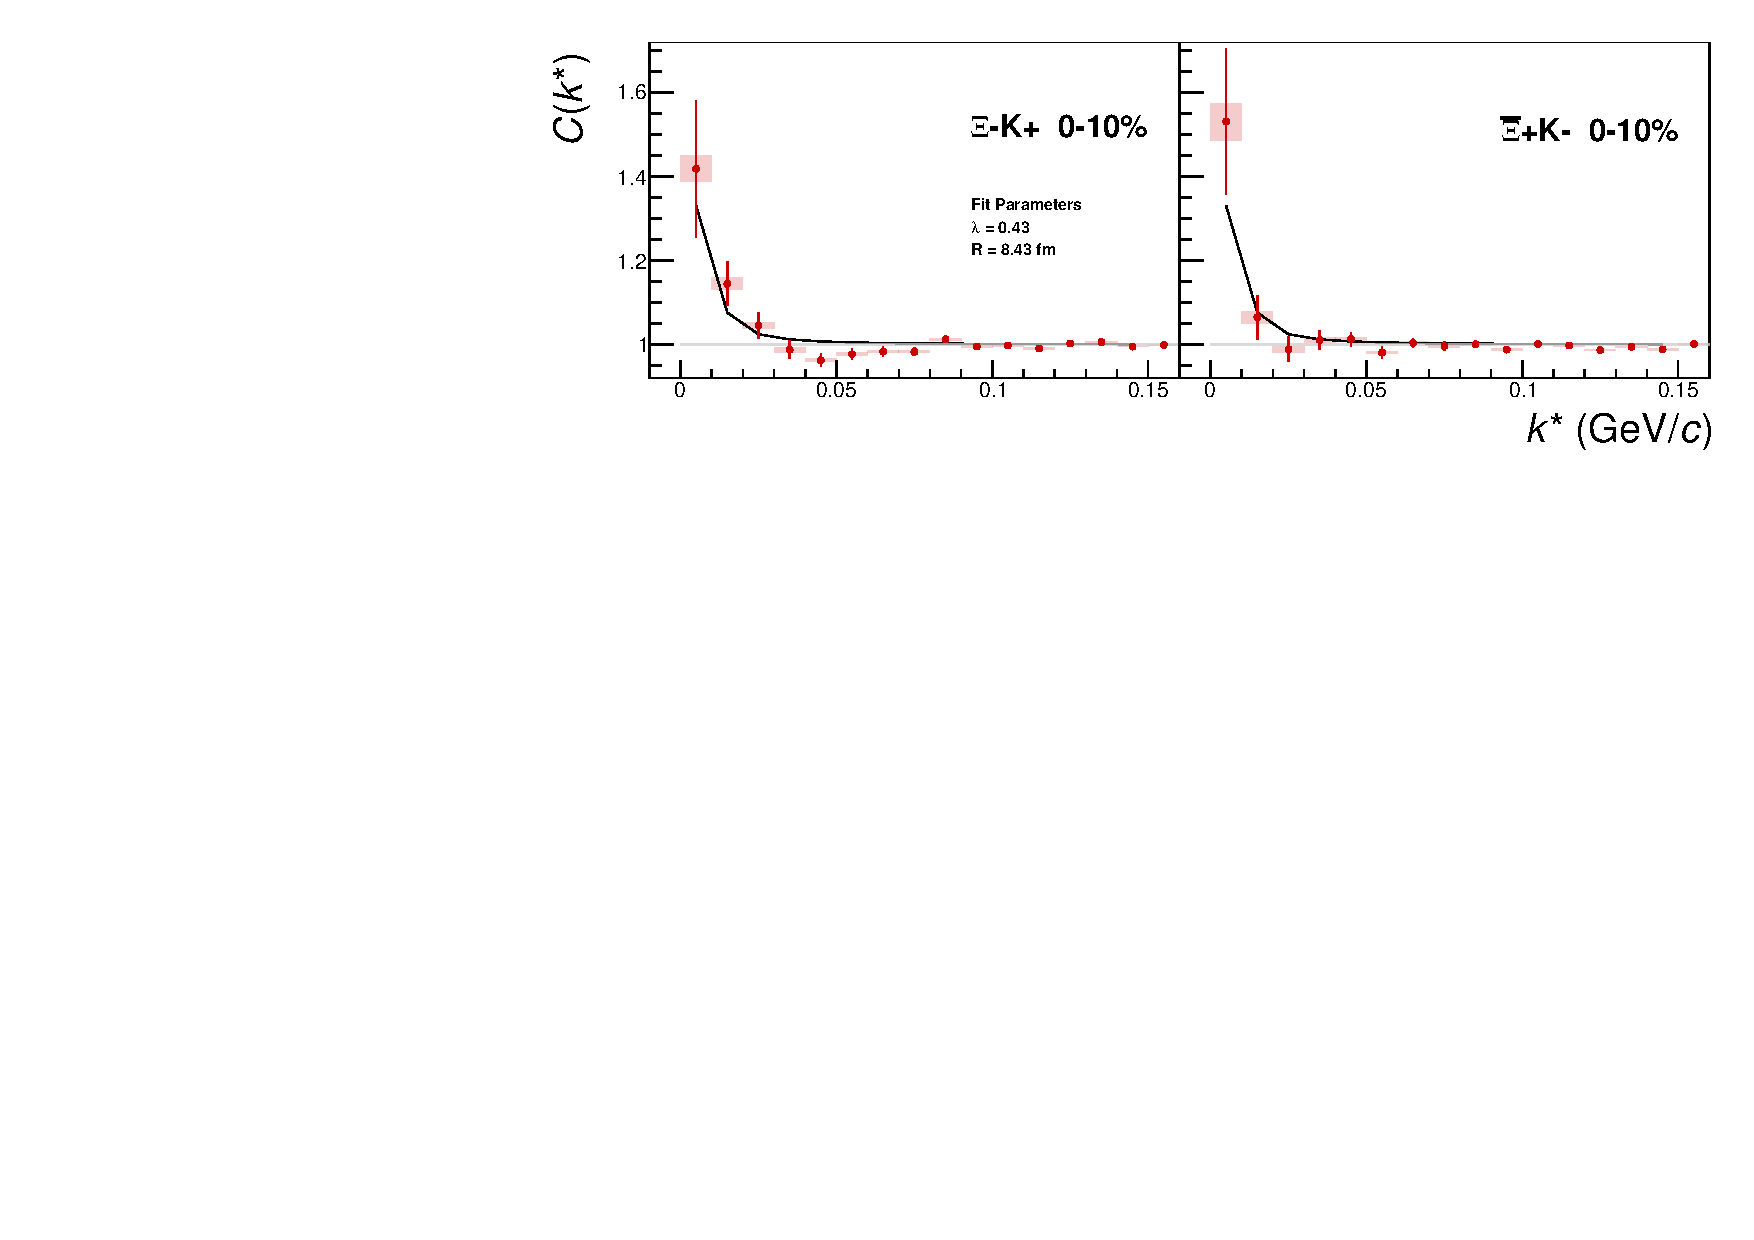
\includegraphics[width=\textwidth]{7_ResultsAndDiscussion/Figures/CoulombOnlyFitXiKchP_0010.pdf}
  \caption[$\Xi^{-}$K$^{+}$ Coulomb-Only Fit]{$\Xi^{-}$K$^{+}$ Coulomb-only fit for 0-10\% centrality}
  \label{fig:XiKchPCoulombOnlyFit}
\end{figure}

\begin{figure}[h]
  \centering
  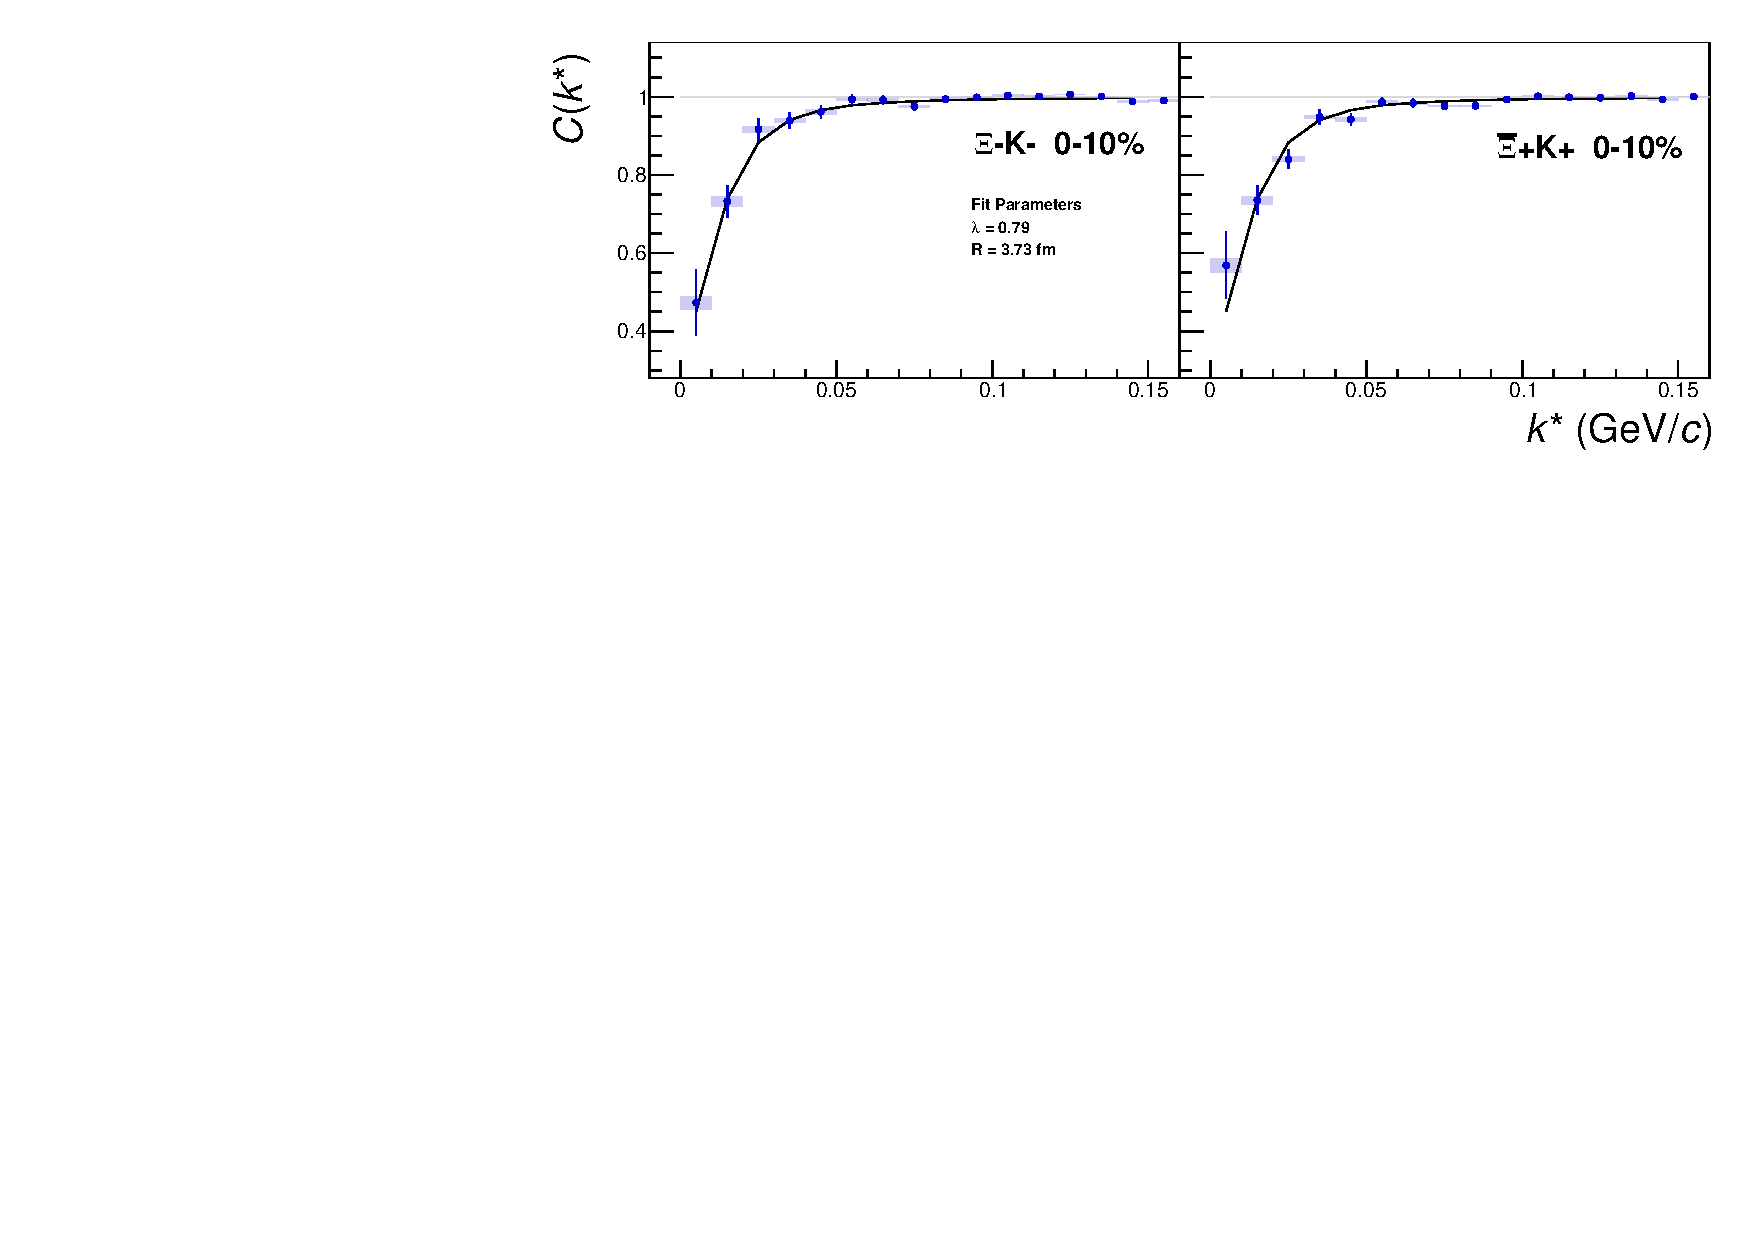
\includegraphics[width=\textwidth]{7_ResultsAndDiscussion/Figures/CoulombOnlyFitXiKchM_0010.pdf}
  \caption[$\Xi^{-}$K$^{-}$ Coulomb-Only Fit]{$\Xi^{-}$K$^{-}$ Coulomb-only fit for 0-10\% centrality}
  \label{fig:XiKchMCoulombOnlyFit}
\end{figure}


\end{document}